
\section{Preliminaries}\label{sec::2.1}

% Threshold models relying on the \emph{Peaks-Over-Threshold} (POT) method propose an alternative to the blocking method seen in the \hyperref[sec::1]{previous Chapter}. This method consider a natural way of determining whether an observation is extreme or not, by focusing only on all observations that are greater than a pre-specified \emph{threshold}. 
% Whereas POT brings problem for the independence (cold days are more likely to be followed by cold days, etc ; more details will be given in \hyperref[sec::3]{Chapter \textbf{\ref{sec::3}}}) and ask the difficult task of choosing the threshold, it avoids the problem of choosing only one observation per block of data which can be a wasteful approach if other "extremes" occur at the same period. The notion of "extremes" is now intrinsically different.
Threshold models relying on the \emph{Peaks-Over-Threshold} (POT) method propose an alternative to the blocking method seen in the \hyperref[sec::1]{previous Chapter}. Focusing exclusively on observations greater than a pre-specified \emph{threshold} provides a natural way to expose extreme values. POT solves the issue of choosing a single observation per data block, but makes the trade-off at the expense of threshold determination and independence issues since cold days are more likely to be followed by cold days, etc ; more details follow in \hyperref[sec::3]{Chapter \textbf{\ref{sec::3}}}. The notion of "extremes" is therefore intrinsically different.


\begin{wrapfigure}{R}{0.4\textwidth}
	\centering
	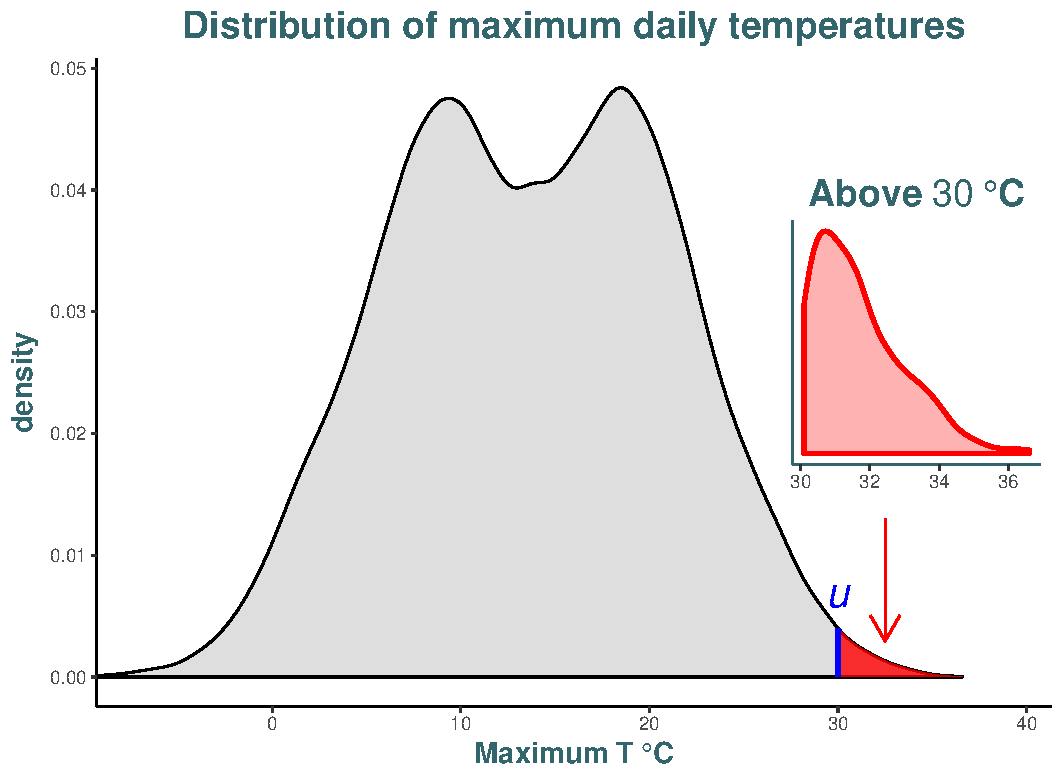
\includegraphics[width=0.4\textwidth]{pot_plot.pdf} % 6.64x5.17 inches
	\caption{Kernel density estimates for the whole series (grey) and for the series of excess over the threshold of $u=30^{\circ} c$ (red). More information on the data will be given in \hyperref[part:xp]{Part \textbf{\ref{part:xp}}}.}
	\label{fig:pot_plot}
\end{wrapfigure}

Let $\{X_j\}$ be a sequence of $n$ iid random variables with marginal df $F$, shown in Figure \textbf{\ref{fig:pot_plot}} representing our application's data. Next we look at observations exceeding a threshold $u$ (blue) that must be lower than the right endpoint (\ref{eq:endpoints}) of $F$. The aim here is to find the child distribution that is depicted in red, say $H$, from the parent distribution $F$ depicted in grey. It will allow us to model the exceedances $Y=X-u$ with $H$ expressed as \begin{equation*}
H(y)=\text{Pr}\{X-u\leq y \ | \ X>u\}.
\end{equation*}
%The kernel density of $H$ is depicted in red in the right plot. 
Throughout this chapter we will aim to model this empirical distribution.

Threshold models can be seen as the conditional survival function of the exceedances $Y$, knowing that the threshold is exceeded, according to \citet[pp.147]{beirlant_statistics_2006} :


\begin{equation}\label{survpar}
\text{Pr}\big\{Y>y\ |\ Y>0\big\}=\text{Pr}\big\{X-u>y\ |\ X>u\big\}=\frac{\bar{F}(u+y)}{\bar{F}(u)}.
\end{equation}
Or similarly, in terms of the exceedance df $F^{[u]}(x)=\text{Pr}\{X\leq u+x \ | \ X>u\}$, see \citet[pp.25-29]{reiss_statistical_2007}
\iffalse
\begin{equation}\label{exceef}
F^{[u]}(x)=\frac{\text{Pr}\{X-u\leq 
	x,X>u\}}{\text{Pr}\{X>u\}}=\frac{F(x+u)-F(u)}{\bar{F}(u)},
\end{equation}
\fi
or following \citet{charras_extreme_2013} and \citet{rosso_extreme_2015}, using the conditional probability law. %Note that (\ref{survpar}) is just the survivor of the exceedance df, namely $\bar{F}^{[u]}$.

If the parent distribution $F$ was known, the threshold exceedances distribution (\ref{survpar}) could be computed. But, as in the method of block maxima, $F$ is unknown in practice. We will still rely on approximations\footnote{We quote here the well-known "\textit{All models are wrong, but some are useful}" from George Box \& Draper (1987), \textit{Empirical model-building and response surfaces}, Wiley, p.424}. Whereas \hyperref[extthm]{Theorem \textbf{\ref{extthm}}} were used to find an approximate distribution for block maxima, we will attempt here to approximate the distribution of the exceedances $H(y)$.


\section{Characterization of the Generalized Pareto Distribution}\label{sec:charac_gpd}

Similarly to the GEV (\ref{gevgen}) in the limit for the block maxima, we look for a limit distribution for exceeding a certain threshold. As for max-stability in \hyperref[maxstab]{Definition \textbf{\ref{maxstab}}}, another formulation can be given for POT models and will help derive a theorem.

\begin{definition}[POT-stability]%\emph{\citet[pp.25]{reiss_statistical_2007}} 
	The dfs $H$ are the only continuous one such that, for a certain choice of constants $a_u$ and $b_u$, 
	\begin{equation*}
	F^{[u]}(a_ux+b_u)=F(x).
	\end{equation*}
\end{definition}
We can now state the key theorem discovered by \citet{balkema_residual_1974} and \citet{iii_statistical_1975-1}.

\begin{theorem}[Pickands–Balkema–de Haan]\label{thm:gpd}
	Let $\{X_j\}$ be the sequence of $n$ iid random variables having marginal df $F$ for which \hyperref[extthm]{Theorem \textbf{\ref{extthm}}} holds. Then,
	\iffalse
	\begin{equation*}
	|F^{[u]}(x)-H_{\xi,\sigma_u}(x)|\longrightarrow 0, \ \ \ \ \ \ \ \qquad \qquad u\to x_*.
	\end{equation*}
	Similarly, 
	\fi
	\begin{equation} \label{gpdconv}
	\text{Pr}\big\{X-u\leq y\ |\ X>u\big\}\longrightarrow H_{\xi,\sigma_u}(y), \ \ \ \ \ \ \ \ \ \ u\to x_*.
	\end{equation}
	It means that for large enough $u$, the df of  $Y=X-u>0$, conditional on $X>u$, is approximately $H_{\xi,\sigma_u}(y)$ where $H_{\xi,\sigma_u}(y)$ is the \emph{Generalized Pareto Distribution} (\emph{GPD}) :
	
	\begin{equation}\label{gpdeq}
	H_{\xi,\sigma_u}(y)=
	\renewcommand{\arraystretch}{0.6}\left\{\begin{array}{@{}l@{\quad}l@{}}
	\ 1-\Big(1+\frac{\xi y}{\sigma_u}\Big)_+^{-\xi^{-1}}, \ \ \ \ \ \  \ \ \xi\neq 0; \\ 
	\vspace{0.0002cm} \\
	\ 1-\exp\Big\{-\frac{y}{\sigma_u}\Big\}, \ \ \ \ \ \ \ \ \ \ \xi=0.
	
	\end{array}\right.\kern-\nulldelimiterspace
	\end{equation}
	
\end{theorem}
%$H_{\xi,\sigma_u}(y)$ is commonly known as the Generalized Pareto Distribution (GPD) 
%and for the approximating GP distribution function possessing the same left endpoint $u$ as the exceedance distribution function $F^{[u]}$
%It means that as the threshold approaches the right endpoint $x_*$ of $F$, is the Generalized Pareto Distribution (\textbf{GPD}) $H_{\xi,\sigma_u}(y)$.
The scale parameter is denoted $\sigma_u$ to emphasize its dependency with the specified threshold $u$ :

\begin{equation}\label{sig1}
\sigma_{u}=\sigma+\xi (u-\mu),
\end{equation}
where we notice the absence of location parameter $\mu$ in (\ref{gpdeq}) as it appears in (\ref{sig1}). 

\subsection{Outline proof of the GPD and justification from GEV}
In the following sections we describe a meaningful yet not too technical way of retrieving the GPD.
%As we also did for block maxima, we think interesting to have a formal and comprehensive, still not too technical, intuitive view of how we retrieved the GPD. %We remind that we aim here at retrieving the GPD $H_{\xi,\sigma_u}(y)$ (\ref{gpdconv}-\ref{gpd}) from probability distributions as expressed in (\ref{survpar}-\ref{exceef}).

\begin{proof}[\boxed{\emph{\textbf{Outline Proof}}}\nopunct ] of \hyperref[extthm]{Theorem \textbf{\ref{thm:gpd}} :} 
	\ \ \ \begin{itemize}
		%\item \fontsize{11pt}{18pt}\selectfont
		\item From \hyperref[extthm]{Theorem \textbf{\ref{extthm}}}, we have for the distribution of the maximum, for large enough $n$,  
		
		\begin{equation}
		F_{X_{(n)}}(z)=F^n(z)\approx \exp\Bigg\{ -\bigg[1+\xi\bigg(\frac{z-\mu}{\sigma}\bigg)\bigg]^{-\xi^{-1}}\Bigg\},
		\end{equation} 
		with $\mu,\sigma>0$ and $\xi$ the GEV parameters. Hence, by taking logarithm on both sides, we get
		
		\begin{equation} \label{logF}
		n \ln F(z)\approx -\Bigg[1+\xi\bigg(\frac{z-\mu}{\sigma}\bigg)\Bigg]^{-\xi^{-1}}.
		\end{equation}
		\item We also have that, from Taylor expansion,
		$\ln F(z)\approx -\big[1-F(z)\big]$
		as both sides go to zero as $z\rightarrow\infty$. Therefore, substituting into (\ref{logF}), we get the following for large $u$ :
		
		\begin{equation*}
		1-F(u\boldsymbol{+y})\approx n^{-1}\bigg[1+\xi\bigg(\frac{u\boldsymbol{+y}-\mu}{\sigma}\bigg)\bigg]^{-\xi^{-1}}.
		\end{equation*}
		where we added the term $\boldsymbol{y}>0$ to retrieve something in the form of 
		(\ref{survpar}). 
		
		\item Finally, by mathematical manipulation, as 
		$u\rightarrow x_*$ :
		
		
		\begin{equation}\label{eq:gpdproof2}
		\begin{aligned}
		\text{Pr}\{X>u+y\ | \ X>u\}
		= \frac{\bar{F}(u+y)}{\bar{F}(u)} 
		& \approx\frac{n^{-1}\big[1+\xi\sigma^{-1}(u+y-\mu)\big]^{-\xi^{-1}}}{n^{-1}\big[1+\xi\sigma^{-1}(u-\mu)\big]^{-\xi^{-1}}} \\  
		& = \bigg[1+\frac{\xi\sigma^{-1}(u+y-\mu)}{1+\xi\sigma^{-1}(u-\mu)}\bigg]^{-\xi^{-1}} \\
		& = \bigg[1+\frac{\xi y}{\sigma_u}\bigg]_+^{-\xi^{-1}},
		\end{aligned}
		\end{equation}
		By simply taking the survivor of (\ref{eq:gpdproof2}), we retrieve 
		
		\begin{equation}
		\begin{aligned}
		\text{Pr}\{X-u\leq y\ | \ X>u\} & =1-\text{Pr}\{X>u+y\ | \ X>u\} \\
		& = 1-\bigg(1+\frac{\xi y}{\sigma_u}\bigg)_+^{-\xi^{-1}},
		\end{aligned}
		\end{equation}
		which is $GPD(\xi,\sigma_u)$ as required.
	\end{itemize}
\end{proof}
More insights come from \citet[pp.27-28]{reiss_statistical_2007} with analysis of rates of convergence. Examples of how to retrieve the GPD from specific distributions are available in \citet[pp.77]{coles_introduction_2001}.


\subsection{Dependence of the scale parameter } We chose to express the scale parameter as $\sigma_u$ to emphasize its dependency with the threshold $u$. If we increase the threshold, say to $u'>u$, then the scale parameter will be adjusted :

\begin{equation} \label{mem}
\sigma_{u'}=\sigma_u+\xi (u'-u),
\end{equation}
and in particular, this adjusted parameter $\sigma_{u'}$ will increase if $\xi>0$ and decrease if $\xi<0$.
If $\xi =0$, there would be no change in the scale parameter\footnote{Consistent with the well-known \emph{memoryless property} of the exponential distribution $H_{0,\sigma_u}$}. 
Also, we consider it noteworthy that as for the GEV, the scale parameter $\sigma_u$ for GPD models
differs from the standard deviation since it governs the “size” of the excess, as mentioned in \citet[pp.20]{AghaKouchak_extremes_2013}.
The issue of threshold selection will be discussed in \hyperref[sec:thresh_selec]{Section \textbf{\ref{sec:thresh_selec}}}.

%We think important to point out the fact that, similarly as for the GEV, the scale parameter $\sigma_u$ for GPD models
%is not the usual standard deviation, but does govern the “size” of the excess, as mentioned in \citet[pp.20]{AghaKouchak_extremes_2013}.
%The issue of threshold selection will be discussed in \hyperref[sec:thresh_selec]{Section \textbf{\ref{sec:thresh_selec}}}.


\subsection{Three different types of GPD : Comparison with GEV} 
One should remark the similarity with the GEV distributions. Indeed, parameters of the GPD of the threshold excesses are uniquely determined by the corresponding GEV parameters of block maxima. Hence, the shape parameter $\xi$ of the GPD is equal to that of the corresponding GEV and, most of all, it is invariant.
In block maxima, the GEV parameters would shift for a different block length, while in POT the GPD parameters are not affected by the choice of the threshold due to the self-compensation arising in (\ref{mem}).% \cite[pp.76]{coles_introduction_2001}

Hence, as for the block-maxima approach, there are also three possible families of the GPD depending on the value of the shape parameter $\xi$ which determines the qualitative behaviour of the corresponding GPD. \cite{hosking_parameter_1987}, \cite{singh_parameter_1995}

\begin{itemize}
	\item \textbf{First} type $H_{0,\sigma_u}(y)$ comes by letting the shape parameter $\xi\rightarrow 0$ in (\ref{gpdeq}), giving :
	
	\begin{equation}\label{gpd0}
	H_{0,\sigma_u}(y)=1-\exp
	\Big(-\frac{y}{\sigma_u}\Big), \ \ \ \ \ \ \ \ \ \ \ y>0.
	\end{equation}
	One can easily notice that it corresponds to an \textbf{exponential} df and hence light-tailed with parameter $1/ \sigma_u$, namely 
	$Y\sim\exp(\sigma_u^{-1})$.
	
	\item \textbf{Second} and \textbf{third} types, i.e. when $\xi<0$ and $\xi>0$ (resp.), differ only by their support : 
	
	\begin{equation}\label{gpdm}
	H_{\xi,\sigma_u}(y)=1-\bigg(1+\frac{\xi y}{\sigma_u}\bigg)^{-\xi^{-1}}, \ \ \ \ \  \ \ \text{for} \ \ \ \begin{cases}
	\ y>0,  \ \ \ \ \ \ \ \ \ \ \ \ \ \ \  \ \ \qquad \ \xi>0; \\
	\  0<y<\sigma_u\cdot|\xi|^{-1}, \ \ \ \  \  \  \xi<0.
	\end{cases}
	\end{equation}
	Therefore, if $\xi>0$ the corresponding GPD is of \textbf{Pareto}-type, hence is heavy-tailed, and has no upper limit while if $\xi<0$, the associated GPD has an upper bound $y_*=u+\sigma_u/|\xi|$ and is then of \textbf{Beta}-type. Special case arise when $\xi=-1$ where the pertaining distribution becomes Uniform$(0,\sigma_u)$, result coming from \citet[pp.186]{grimshaw_computing_1993}.
	
	
\end{itemize}
The \textbf{density} of the GPD is written here as

\begin{equation}\label{densgpd}
h_{\xi,\sigma_u}(y)=\begin{cases}
\frac{1}{\sigma_u}\bigg(1+\xi\frac{y}{\sigma_u}\bigg)^{-\xi^{-1}-1}, \qquad\quad \xi\neq 0; \\
\sigma_u^{-1}\cdot e^{-y},\qquad\qquad\qquad\qquad \xi= 0.
\end{cases}
\end{equation}


In the example of Figure \ref{fig:pot_plot}, we can see that the red density seems to have an upper bound around $36.5^{\circ}c$. thence, we can conclude that this distribution should be of Beta-type. \hyperref[part:xp]{Part \textbf{\ref{part:xp}}} will confirm that $\xi<0$.

After looking at the behaviour of the density of these functions, we will procure a more comprehensive view by defining some examples of how to retrieve these different types of Generalized Pareto Distributions.


\section{Return Levels}\label{sec:rl_gpd}

Presented in \hyperref[rlgev]{Section \textbf{1.6}} for block maxima, return levels are also useful in POT to bring valuable information. 
%From (\ref{gpdeq}), we obtain the quantiles of the GPD simply by setting this equation equal to $1-1/m$ and inverting.
However, unlike for block maxima, the quantiles of the GPD cannot be as readily interpreted as return levels because the observations no longer derive from predetermined \emph{blocks} of equal length. Instead, it is now required to estimate the \emph{probability of exceeding the threshold} $\zeta_u=\text{Pr}\big\{X>u\big\}$, from which a natural estimator is $\hat{\zeta}_u=k/n$ with $k$ the number of points exceeding $u$.
We can now retrieve the return level $r_m$, i.e. the\emph{ value that is exceeded on average once every $m$ observations}. 
This is given by 

\begin{equation}\label{rlpot}
r_m=\begin{cases}
\ u+\sigma_u\ \xi^{-1}\Big[(m\zeta_u)^{\xi}-1\Big], \ \ \ \ \ \ \ \ \  \ \xi\neq 0;\\
\ u +\sigma_u \log(m\zeta_u), \ \quad \ \ \ \ \ \ \  \ \ \ \ \ \ \quad \ \xi =0.
\end{cases}
\end{equation}
provided $m$ is sufficiently large.
Computations are very similar as for the GEV in \hyperref[rlplot]{Section \textbf{\ref{rlplot}}}. 

\subsubsection*{Interpretation}

Whereas the interpretation of the plot in function of the shape parameter value is the same as for the block-maxima method (see \hyperref[rlplot]{Section \textbf{1.8}}), it is more convenient to replace the value of $m$ by $N\cdot n_y$ in (\ref{rlpot}), where $n_y$ is the number of observations per year, to give return levels on an annual scale. This method allows us to obtain the\emph{ N-year return level} which is now commonly defined as the level expected to be exceeded once every $N$ years.

\iffalse
\section{Point Process Approach}\label{poissonproc}
[coles, pp.124] Here, Point Process could be seen as a kind of summary of the two previous methods (respectively in \hyperref[sec::1]{Chapter \textbf{1}} and in rest of \hyperref[sec::2]{this Chapter}), leading to nothing new. However, this approach if often preferred as : %for his "flexibility" 
\begin{enumerate}
	\item Its interpretation \textbf{unifies} the \textbf{models} considered so far.
	\item Its likelihood enables a more natural formulation of non-stationarity in excess models from the Generalized Pareto model, see section \textbf{2.2}.
\end{enumerate}
Furthermore, we will see that the parametrization of the point process model is invariant to threshold choice %[p.136] 
so that this variation would only affect the well-known (already mentioned) bias-variance trade-off in the inference. Interesting if seasonal modelling.

Hence, we recall that if $Y$ is Poisson distributed with parameter $\lambda$, then 

\begin{equation}\label{poissdist}
\text{Pr}\big[Y=k\big]= e^{-\lambda}\frac{\lambda^k}{k!}, \qquad\quad k\in\mathbb{N.}
\end{equation}

\subsection{Non-homogeneous Poisson Process} 

\begin{equation}
N(A)\sim \text{Poi}(\Lambda(A)), \ \ \ \ \ \ \ \,\ \ \ \ \Lambda (A) = \int_A \lambda (x)dx.
\end{equation}

"If a process is stationary and satisfies an asymptotic
lack of “clustering” condition for values that exceed a high threshold, then its limiting form is
non-homogeneous Poisson with intensity measure" $\Lambda$, on a set of the form $A = (t_1,t_2)\times (x,\infty)$, given by 

\begin{equation}
\Lambda(A) = (t_2-t_1)\cdot\bigg[1+\xi\bigg(\frac{x-\mu}{\sigma}\bigg)\bigg]^{-\xi^{-1}}_+
\end{equation}
\fi 

\section{Inference : Parameter Estimation}\label{sec::potinfernce} 

We will not develop likelihood techniques here as is ressembles that of GEV in \hyperref[sec::gevinfernce]{Section \textbf{\ref{sec::gevinfernce}}}, and requires numerical techniques as well. 


The two approaches we have encountered so far, i.e. block-maxima and POT share the same parameter $\xi$. Therefore, it is not necessary to differentiate between these methods for the sole estimate of the shape parameter. We give in \hyperref[sec:infevi]{Appendix \textbf{\ref{sec:infevi}}} some of the most used methods to estimate the EVI.


\iffalse
\subsection{Likelihood-based Methods}\label{likintro_pot}



\subsection*{Generalized Pareto Distribution}

As we have seen, excess-over-threshold models rely on ....
From (\ref{densgpd}), we can write the \emph{log-likelihood }of the GPD : 

\begin{equation}\label{likk}
\ell(\textbf{z};\xi,\sigma_u) = -n\ln\sigma_u-(1+\xi^{-1})\sum_{i}^n\ln(1+\xi \sigma_u^{-1}z_i), \ \ \ \ \ \ \ \ (1+\xi \sigma_u^{-1}z_i)>0.
\end{equation}


\subsection{Profile Likelihood}

\subsection{Other Methods}

\fi


Finally, methods dedicated to POT exist to estimate the parameters of the GPD. For example, they can include the probability-weighted-moment (PWM) which is formulated differently as for GEV in \hyperref[sec:gevother]{Section \textbf{\ref{sec:gevother}}}, see e.g. 
\citet{ribereau_skew_2016}. The $L$-moment estimator is also important, especially for rainfall application, where \cite{hosking_regional_1997} emphasized that $L$-moment method came historically as a modification of the PWM estimator.



\section{Inference : Threshold Selection }\label{sec:thresh_selec}

Threshold selection is crucial in a POT context.
It involves a \emph{bias-variance trade-off}, that is :

\begin{itemize}
	\item \emph{Lower threshold} will induce\emph{ higher bias} due to model mispecification. In other words, the threshold must be sufficiently high to ensure that the asymptotics underlying the GPD approximation are reliable.
	
	\item \emph{Higher threshold} will imply higher estimation uncertainty, i.e. \emph{higher variance} of the parameter estimate as the sample size is reduced for high threshold. 
	
\end{itemize}



\subsection{Standard Threshold Selection Methods}

%(Following \cite{leadbetter_extremes_1983}, this is practically equivalent to estimation of the $k^{\text{th}}$ upper order statistic $X_{(n-k+1)}$called the "tail fraction" below. To ensure tail convergence, as $n\to\infty$, $k\to\infty$ but at a reduced rate such that $k/n\to 0$, i.e. the quantile level of the threshold increases at a faster rate as the sample size $n$ grows. )

Applications of all the subsequent methods can be viewed in Section 3.1 of the \textbf{Summary1\_intro.Rmd} in the \textbf{/vignettes} folder of the \href{https://github.com/proto4426/PissoortThesis/tree/master/vignettes}{repository}. %\footnote{See \hyperref[appgit]{Appendix \textbf{\ref{appgit}}} or you can go directly to \url{https://github.com/proto4426/PissoortThesis/tree/master/vignettes}. More details will come in \hyperref[part:xp]{Part \textbf{\ref{part:xp}}}. }. 
Vignette can be downloaded in html from the compressed file in the same folder. Recall that all empirical results of this chapter will not be included in this thesis.

\subsubsection*{Based on Mean Residual Life}
The \emph{mean residual life} function or \emph{mean excess} function is defined as

\begin{equation}
%\begin{aligned}
mrl(u_0)
:=E(X-u_0\ |\ X>u_0) 
\ = \frac{\int_{u_0}^{x_*} \bar{F}(u)du}{\bar{F}(u_0)},
%\end{aligned}
\end{equation}
for $X$ having survival function $\bar{F}(u_0)$ computed at $u_0$.
It denotes in an actuarial context
the expected remaining quantity or amount to be paid out when a level $u_0$ has been chosen. However, there are also interesting and reliable applications in an environmental context.
Moreover, this function yields valuable properties about the tail of the underlying distribution of $X$. In fact, we expect that :

\begin{itemize}
	\item If $mrl(u_0)$ is constant, then $X$ is exponentially distributed.
	\item If $mrl(u_0)$ ultimately increases, then $X$ has a heavier tail than the exponential distribution.
	\item If $mrl(u_0)$ ultimately decreases, then $X$ has a lighter tail than the exponential distribution.
\end{itemize}
% (and vice-ersa, goes it in the two sens??)
This can be particularly interesting for our purpose when considering threshold models. For this case, we have the excesses $\{Y_i\}$ that follow a GPD (\ref{gpdeq}) and which are generated by the sequence $\{X_i\}$. From the theoretical mean of this distribution, we retrieve  (provided $\xi<1$)

\begin{equation} \label{mrl}
\begin{aligned}
mrl(u):=E(X-u\ |\ X>u)
& = \frac{\sigma_u}{1-\xi} \\
& = \frac{\sigma_{u_0}+\xi u}{1-\xi},
\end{aligned}
\end{equation}
from dependence of the scale parameter $\sigma$ with the threshold $u$, see (\ref{mem}). Hence, we remark that $mrl(u)$ is linearly increasing in $u$, with gradient $\xi\cdot(1-\xi)^{-1}$ and intercept $\sigma_{u_0}\cdot (1-\xi)^{-1}$. Furthermore, we can estimate empirically this function by 

\begin{equation}\label{mrle}
\widehat{mrl}(u)=\frac{1}{n_u}\sum_{i=1}^{n_u}(x_{[i]}-u),
\end{equation}
where the $x_{[i]}$ denote the i-th observations out of the $n_u$ that exceed $u$.

\paragraph*{Mean residual life plot} 
The \emph{mean residual life plot} results from combining the linearity detected between $mrl(u)$ and $u$ in (\ref{mrl}) with (\ref{mrle}). Therefore, worthwhile information can be retrieved from the locus of the points : 

\begin{equation}
\Bigg\{\bigg(u,\frac{1}{n_u}\sum_{i=1}^{n_u}(x_{[i]}-u)\bigg):u<x_{max}\Bigg\}.
\end{equation}
Even if its interpretation is not straightforward, this graphical procedure will give insights for the choice of a suitable threshold $u_0$ to model extremes via a GPD, that is the threshold $u_0$ above which we can detect linearity in the plot. Relying on this well-chosen threshold $u_0$, the GPD approximation should be correct, even though its interpretation is subjective. Furthermore, information in the far right-hand-side of this plot is unreliable. Variability is high due to the limited amount of data above high thresholds. %This can be seen for example on larger confidence intervals.


%Substantial subjectivity in interpreting thesediagnostic plots, and the resulting uncertainty. Similar challenges are seen withthe River Nidd data, shown in Tancredi et al. (2006), and many other exam-ples in the literature. These examples suggests that a more ‘objective’ thresh-old estimation approach is needed and that uncertainty must be accounted for."   see mixture pdf]

\subsection*{Based on the stability of the parameter's estimates}
%see section 4.3.4 of coles.

%montrer pr varying threshold si les estimateurs changent bcp ?  Stability plots avec IC grisé qui sajuste complement ds cette region.

Due to its simplicity,  \textit{stability plots of the parameter's estimates} is one of the preferred tools for practitioners.
The aim is to plot MLE's of the parameters against different values for the threshold. In theory, MLE's are independent of the threshold choice, and hence the threshold is chosen at the lowest value for which the MLE's remain near-constant. 

But this method is also criticized, especially owing to its lack of interpretability, and the pointwise confidence interval strongly dependent across the range of thresholds.
Other techniques have thus been proposed, see e.g. \citet{Wadsworth_exploiting_2016} which suggests complementary plots with greater interpretability, with a likelihood-based procedure allowing for automated and a more formal threshold selection.
In short, this new method relies on the independent-increments
structure of MLE and makes use of likelihood ratio tests to identify the threshold that significantly provides the best fit to the data. Thresholds are then compared iteratively, and significance is assessed by simulations.

%"To identify a treshold that provides the best fit to the likelihood (8)", we maximize the profile likelihood $L_p(j)=L(\hat{\beta}_j,\hat{\gamma}_j,j)$, with $(\hat{\beta}_j,\hat{\gamma}_j)$ the MLE's for a fixed j. After computing $j^*=\argmaxD_j L_p(j)$, the question is whether $L(\hat{«\beta}_{j^*},\hat{\gamma}_j,j^*$ provides a significantly better fit to $\xi*$ than $L(0,1,0)=\prod_{i=1}^{k-1}\phi(\xi_i^*;0,1)$. This can be answered by a likelihood ratio test, with test statistic \begin{equation} T=\frac{L(\hat{\beta}_{j^*},\hat{\gamma}_{j^*},j^*)}{L(0,1,0)}. \end{equation}
%If this is significant at level $\alpha$, there is evidence against a hypothesis of white noise and then we select the threshold $u^*=u_{j^*+1}$ which provides the best fit.

%"The lowest threshold that one entertains, u1, may also have an impact upon the selected threshold, and might thus be regarded as a tuning parameter. "

%"how many thresholds k one should choose. There should be some link to the sample size of the data: if k is too large compared to the sample size n, then the asymptotic theory will not provide a good approximation to the distribution."



\subsection*{Based on the Dispersion Index Plot}

As mentioned, methods considered above involve substantial amount of subjectivity.
Following \citet{ribatet_users_2006}, the \emph{Dispersion Index} (DI) plot is particularly useful for time series. Point process that we have not developed here, can be used to characterize the excess over a threshold as a Poisson process. Hence, $\mathbb{E}[X]=\text{Var}[X]$. The DI statistic introduced by \cite{cunnane_note_1979} is 
defined by $DI=s^2\cdot\lambda{-1}$, where $s^2$ is the intensity of the Poisson process and $\lambda$ is the mean number of events in a block.


\subsection*{Based on \emph{L}-Moments plot}

\emph{L-Moments} are linear combinations of the ordered data values. 
From the GPD, we have that

\begin{equation}
\tau_4=\tau_3\cdot \frac{1+5\tau_3}{5+\tau_3},
\end{equation}
where $\tau_4$ is the \emph{L-Kurtosis} and $\tau_3$ is the \emph{L-Skewness}. See e.g. \citet{hosking_regional_1997} for more details on L-moments or \citet{peel_utility_2001} for a known application of this method in hydrology.

We can then construct the \emph{L-Moment plot} which consist of the points :

\begin{equation}
\Big\{(\hat{\tau}_{3,u},\hat{\tau}_{4,u}) : u\leq x_{\text{max}}\Big\}
\end{equation}
where $\hat{\tau}_{3,u}$ and $\hat{\tau}_{4,u}$ are estimations of L-kurtosis and L-skewness based on $u$ and $x_{\text{max}}$ is the maximum observation. Note that interpretation of this plot is often tedious.






\subsection{Varying Threshold : Mixture Models}

The so-called "fixed threshold" approaches (as renamed in 
\citet{scarrott_review_2012}, among others) considered so far have been criticized since it leads to a fixed and subjective threshold, sometimes also seen as an arbitrary choice where the uncertainty cannot be taken into account. 

%The so-called "fixed threshold" approaches (as renamed in \citet{scarrott_review_2012}, among others) loosely defined such that the population tail can be well approximated by the GPD, obtaining a balance between the bias due to the asymptotic tail approximation and parameter estimation uncertainty due to the inherent sparsity of threshold excess data.


Hence, recent models have emerged that allow a dynamic view of the threshold. In \textit{mixture models}, the threshold is either implicitly or explicitly defined as a parameter to be estimated, and in most cases the uncertainty associated with the threshold choice can be naturally accounted for in the inferences. The model can be presented in a general way : 

\begin{equation}
f(x)=(1-\zeta_u)\cdot b_t(x)+\zeta_u\cdot g(x),
\end{equation}
where $\zeta_u=\text{Pr}\big\{X>u\big\}$ is now called the \emph{tail fraction} and is a new parameter of the model, $b_t(x)$ is the density of the \textit{bulk model} (i.e., the data that does not exceed the threshold) and $g(x)$ is the \emph{tail model}, e.g. the GPD density. We ignored parameter dependence for clarity. There is abundant literature on the subject and numerous models have emerged, not necessarily parametric, see e.g. \citet[chap.3]{dey_extreme_2016} for the univariate case.
The guiding principle in choosing EV mixture models is to combine a flexible bulk model with a reliable tail fit which is robust to the bulk data. These two components are not independent as they share common information about the threshold.

Serious issues arise in these models, for example regarding the discontinuity that often occurs in the density function at the junction between the bulk and the tail model. Alternative models have emerged to force continuity on the density but still, mixture models are often regarded as over-complex with respect to the benefits these models can offer in practice. Research is in great progress but we think improvements have still to be made before yielding straightforward modeling and valuable results.


\iffalse
A Problem involves the discontinuity which often occur in the density function. this can present bias and uncertainty when the quantity of interest considered is close to the threshold.
"Nonstationary extensions of such models can be particularly problematic
with the extent of discontinuity varying along the threshold function."

Alternatives are possible to force continuity on the pdf.

"If the bulk model is correctly specified, then the parametric
mixture models are easy to understand and quick to fit so are
preferred. However, in more usual situation of unknown
population distribution, the nonparametric mixture models
perform consistently well for low and high quantiles." evmix package thesis.

Nonstationary extremes see thesis2012 p.155

A huge debate and more information can be found in \citet[chap.3-5]{dey_extreme_2016}.

\paragraph*{Cross-validation}
\cite{northrop_cross-validatory_2017} 
Besides all these methods that are very subjective,...
%or see gelman bayesian book pp.169

\fi